\documentclass[11pt]{article}
\usepackage{geometry} % see geometry.pdf on how to lay out the page. There's lots.
\usepackage{hyperref}
\usepackage{graphicx}
\usepackage{gensymb}
\usepackage[affil-it]{authblk}
\usepackage[toc,page]{appendix}
\usepackage{pifont}
\usepackage{amsmath}
\usepackage{amsthm}

\usepackage{float}

\newtheorem{theorem}{Theorem}[section]
\newtheorem{conjecture}[theorem]{Conjecture}
%% \usepackage{draftwatermark}

%% \SetWatermarkText{DRAFT}
%% \SetWatermarkScale{6}
%% \SetWatermarkLightness{0.95}

% \geometry{letter} % or letter or a5paper or ... etc
% \geometry{landscape} % rotated page geometry

% See the ``Article customise'' template for come common customisations

\title{Untwisting a Tetrahelix}
\author{Robert L. Read
  \thanks{read.robert@gmail.com}
}
\affil{Founder, Public Invention, an educational non-profit.}


\date{\today}

%%% BEGIN DOCUMENT
\begin{document}

\maketitle

%% \tableofcontents

\begin{abstract}
  By using irregular tetrahedra, one can transform a tetrahelix into a spaceframe that is not twisted, forming a ``tetrabeam''.
  In the case of an equilateral profile, an analytic set of members lengths is provided which are shown to be optimal.
  This tetrabeam is formed with only three member lengths ($\sqrt{13/9}, \sqrt{10/9}$, and $1$.) 
\end{abstract}


\section{Introduction}

The Boerdijk--Coxeter helix is a stack of tetrahedra face to face that winds about a straight line. The vertices of the tetrahedra
lie upon three
helices about the central axes. The Tetrobot/Glussbot project
uses this regularity of this geometry to make a tentacle-like robot that can move like a slug or mollusc. The Tetrobot concept
is to use mechanical members, called actuators, which can change their length, connected by special joints which allow many
members to come to a single point. Such machines can follow purely mathematical models such as the Boerdijk–Coxeter helix or the Octet Truss.

However, a tetrahelix does not rest on a plane in a simple way. It is convenient to have it ``untwist'' and form a spaceframe that
has a flat planar surface. By making length changes in a certain way, we can untwist a tetrahelix to form a ``tetrabean'' which
is perfectly flat and has, for example, an equilateral triangular profile.

\section{Approach}

A tetrahelix has the useful property that every member is precisely the same length. If we relax this, so that the tetrahedra it
comprises are not perfectly regular, then we can twist and curve the tetrahelix into a variety of shapes. This is useful to
the mechanical engineer or robotocists because the structure remains an inherently rigid, omni-triangulated space frame, which
may be expected to be at least somewhat mechanically strong.

In particular, we can untwist the perfectly regular tetrahelix to form a ``tetrabeam''. We seek a tetrabeam that is irregular
(in terms of its tetrahedra) but regular enough in terms of mechanical engineering to be comprehensible and computationally tractable.
Observe that a regular tetrahelix appears to have three bumpy ``tracks'' which wind about the central axis.  We seek to unwind
these tracks so each track is a plane.

In order to do this for an tetrahelix of arbitrary length, we need a nameing convention for each member. We propose a coloring
scheme in which the joints and members on the outer ``rails'' of the tetrahelix are colored in primary colors red, yellow and blue.
We propse that the interior members be colored based on the rails they connect using an additive color scheme, or orange, purple, and green,
if the member connects red to yellow, red to blue, or blue to yellow, respectively.  Furthermore, we call interor members ``even'' if they
are even numbered starting from the joint at the origin, and ``odd'' if they are odd-numbered.  We have found that nine classes thus
formed are sufficient to untwist the tetrahelix and for our purposes: $red, yellow, orange_{even}, orange_o, purple_e, purple_o, green_e, green_o$. In the diagram below, the ``odd'' members are draw with a dashed line.


 \begin{figure}[H]
     \centering
     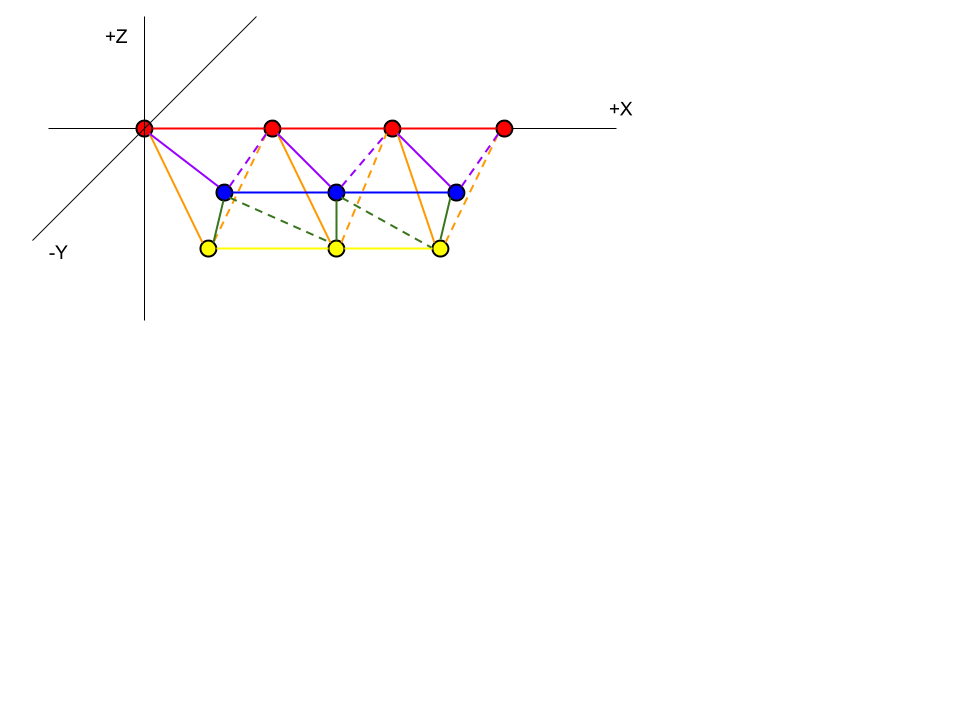
\includegraphics[width=0.5\textwidth]{TetrahelixColoringDiagram.png}
     \caption{Coloring of an (untwisted) Tetrabeam}
 \end{figure}

 Having observed that the tetrahelix can form a tetrabeam, we need merely compute the length of the member classes.

 Although one could choose any beam width and beam height in principle, and a structural engineer would like choose a ``deep'' beam that had
 a height greater than its width, our primary motivation is support the Tetrobot, which uses members that all have the same maximum and
 minimum length. It therefore is sensible to consider a ``tetrabeam'' with the cross-sectional profile of an equilateral triangle.
 Furthermore, acting as robotics engineers we seek to have all members to be similar in length, because this allows us the greatest
 flexibility in making the tetrabeam crawl, or walk, or curl, topics outside the scope of this paper.

 If we simply constrain all red joints to the origin and all blue joints to a line parallel to the x-axis at the vertix of an equilateral
 triangle descending from the origin, we will have simple equations in Cartesian space. We use the variable B to mean the x coordinate
 of the $blue_0$ node and Y to mean the x-cordnate of the $yellow_0$ node. Since for our purposes we do not need distance but rather relative distances
 until our last step, we organize these equations as \emph{quadrances}, leaving both sides of the equations squared.
 We further assume the red, yellow and blue members are all unity. The alitude of an equilateral triangle is $\sqrt{3}/2$.
 These equations follow from the distance formula in three space.
 \begin{align*}
   D^2 &= (\Delta z)^2 + (\Delta y)^2 + (\Delta x)^2 \\
 orange_e^2 &= (\sqrt{3}/2)^2 + (1/2)^2 + Y^2 & &= 1 + Y^2\\
 orange_o^2 &= (\sqrt{3}/2)^2 + (1/2)^2 + (1-Y)^2 & &= 1 + (1-Y)^2\\
 purple_e^2 &= (\sqrt{3}/2)^2 + (1/2)^2 + B^2 & &= 1 + B^2\\
 purple_o^2 &= (\sqrt{3}/2)^2 + (1/2)^2 + (1-B)^2 & &=  1+ (1-B)^2\\
 green_e^2 &= (B - Y)^2 + 1^2 + 0^2 & &= 1 + (B - Y)^2 \\ 
 green_o^2 &= ((1+Y) - B)^2 + 1^2 + 0^2 & &= 1 + ((1+Y) - B)^2 \\ 
\end{align*}

 We then ask the question: what are useful values for B and Y, from which we will have constrained and computed the lengths of all
 members.

 \section{Choosing the parameters}

 Choices of $Y$ and $B$ correspond to slideing the yellow and blue rail relative to the red rail. However, we seek to choose them such that all
 classes of members have similar lengths. In particular, we want to minimize the difference between the shortest and longest.

 It particular we have no interest in solutions in which these rails swing past the $red_1$, or swing behind $red_0$, so we
 assert $0 \leq Y \leq 1$ and $0 \leq B \leq 1$. Without loss of generality, let us choose that $Y$ will be the at least as close to the origin as $B$,
 so $Y  < B$.

 We investigate possible choices of $Y$ and $B$ numerically with a computer before observing the apparent result that the maximum distance in
 length is minimized when $Y = 1/3$ and $B = 2/3$.

 \begin{theorem}
Let $f$ be a function whose derivative exists in every point, then $f$ is 
a continuous function.
\end{theorem}

 \begin{proof}
   Assume that $1 = Y + B$.  I don't have a great argument for this at present.

   Assume that $Y < 1/2$. Then $B > 1/2$. Substituing $1 - Y$ for $B$ in our equations:
 \begin{align*}
   orange_e^2 &= 1 + Y^2 \\
 orange_o^2 &= 1 + (1-Y)^2 \\
 purple_e^2 &=  1 + (1-Y)^2 \\
 purple_o^2 &=   1+ (1-B)^2 & &= (1 + (1 - (1 - Y))^2 & & = 1 + Y^2 \\
 green_e^2 &=  1 + (B - Y)^2 & &= (1 - ((1 - Y - Y)^2)) & &= 1 + (1 - 2Y)^2\\ 
 green_o^2 &= 1 + ((1+Y) - B)^2 & &= 1 + ((1+Y) - (1 - Y))^2 & &= 1 + (2Y)^2 \\
 \end{align*}

 Now assume $green_o$ and $orange_o$ are the two largest of these values, so that we minimize the entire group by setting them equal.
 Then:
\begin{align*}
  green_o^2 &= orange_o^2 \\
  1 + (2Y)^2 &= 1 + (1-Y)^2 \\
  4Y^2 = 1 + -2Y + Y^2 \\
  3Y^2 + 2Y - 1 = 0 \\
\end{align*}
Which has two solutions, $Y = -1$, which we throw out because we assumed $0 \leq Y$, and $Y = 1/3$.

Therefore $Y = 1/3$ minimizes the length difference of all members.
 \end{proof}

Our complete solution is therefore:
\begin{align*}
  Y &= 1/3 \\
  B &= 2/3 \\  
   orange_e &= \sqrt{1 + (1/3)^2} & &= \sqrt{10/9} \\
 orange_o &= \sqrt{1 + (1-1/3)^2} & &= \sqrt{13/9} \\
 purple_e &=  orange_o  \\
 purple_o &=  orange_e \\
 green_e &=  \sqrt{ 1 + (1 - 2/3)^2} & &= \sqrt{10/9} \\ 
 green_o &=  \sqrt{1 + (2/3)^2} & &= \sqrt{13/9} \\
 \end{align*}
So in fact we can construct a tetrabeam using only three member lengths $1$,
$\sqrt{10/9} = 1.05409\cdots$, and $\sqrt{13/9} = 1.20185\cdots$.
In other words, our longest members is only 21\% longer than our shortest member.
As it happens, the current Tetrobot implementation can support about a 50\%
change in length, so it can easily realize this Tetrabeam configuration. If one were
to construct a static tetrabeam by welding, this limit number of member lengths would be convenient.
 
 
\section{Open Questions}

I hardly dare claim these to be ``open questions'', yet they are questions of interest to the Tetrobot/Glussbot project.

\begin{conjecture}

  Using the six member classes defined by the non-primary colors, it is possible to smoothly twist and untwist a tetrahelix.
  
  \end{conjecture}



\section{Contact and Getting Involved}

The Gluss Project \url{http://pubinv.github.io/gluss/}
is a free-libre, open-source research, hardware, and software project that welcomes volunteers.
It is our goal to organize projects for the benefit of all humanity without seeking profit or intellectual property.
To assist, contact \href{mailto:read.robert@gmail.com}{$<$read.robert@gmail.com$>$}.

\bibliographystyle{IEEEtran}
\bibliography{IEEEabrv,gluss}

\end{document}

